\documentclass[10pt,a4paper]{article}
\usepackage[margin=2.2cm]{geometry}
\usepackage{fontspec}
\usepackage{kotex}
\setmainfont{Apple SD Gothic Neo}
\setsansfont{Apple SD Gothic Neo}
\usepackage{amsmath,amssymb}
\usepackage{graphicx}
\usepackage{booktabs}
\usepackage{caption}
\usepackage[dvipsnames]{xcolor}
\usepackage[colorlinks=true,linkcolor=MidnightBlue,citecolor=MidnightBlue,
            urlcolor=MidnightBlue]{hyperref}
\usepackage{titlesec}
\titleformat{\section}{\large\bfseries}{\thesection}{0.6em}{}
\titleformat{\subsection}{\normalsize\bfseries}{\thesubsection}{0.5em}{}
\captionsetup{font=small,labelfont=bf}
\setlength{\parskip}{0.35em}
\setlength{\parindent}{0pt}

\usepackage{mdframed}
\newmdenv[linewidth=0.4pt,linecolor=gray!60,backgroundcolor=gray!5,
          innertopmargin=6pt,innerbottommargin=6pt,skipabove=8pt,skipbelow=8pt]{claimbox}
\newcommand{\claim}[2]{\begin{claimbox}\textbf{주장.} #1\par\smallskip
  \textcolor{gray!70}{\textbf{반증 조건.} #2}\end{claimbox}}

\title{\bfseries 첫 면허\\[2pt]
\large 새 씨앗이 재현했고, 좁은 문 하나를 정식으로 열었다}
\author{월드모델 실험실 · 노트 $802$}
\date{2026-08-07}
\begin{document}\maketitle

\section{한 줄}

논문 $165$ 가 멈춘 자리에서 확인 측정을 돌렸다 --- \textbf{목록은 못박혀 있었고}
($8$개 도메인 · 가용성이 정한 것), \textbf{씨앗은 새것}($4{\sim}7$)이고,
\textbf{동점띠는 실용 폭}($0.01$ · 규약 $46$)이었다.

\begin{center}
\begin{tabular}{lrr}
\toprule
$8$개 판 가중(행 $3{,}015$) & 자릿수 오차 & \\
\midrule
\textbf{B 드리프트 보정} & $\mathbf{0.1430}$ & 씨앗별 $0.1420{\sim}0.1449$ \\
C 기후값 & $0.1675$ & \\
\midrule
\textbf{B$-$C} & $\mathbf{-0.0245}$ & 동점띠의 $2.45$배 · $801$ 의 $-0.0241$ 재현 \\
\bottomrule
\end{tabular}
\end{center}

\textbf{판정 (가) --- 조건부 능력 승격.} 능력 카드의 여섯째 허용 꼴이 생겼다:
\emph{드리프트 보정 절대값 --- $8$개 도메인 한정 · 자와 함께.} 노트 $691$ 이후
\textbf{한 건씩 절대값으로는 처음이다.}

\begin{figure}[t]\centering
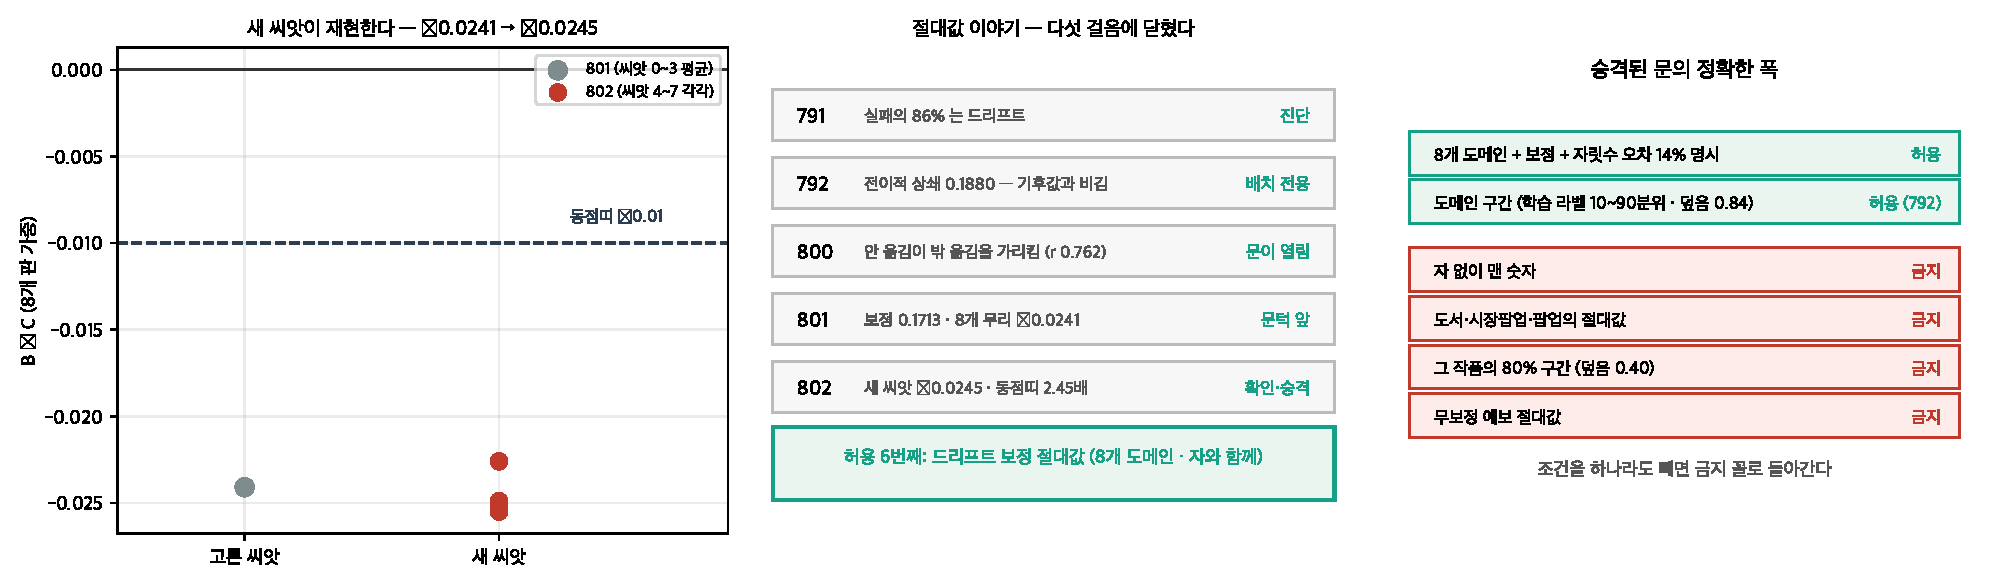
\includegraphics[width=0.99\textwidth]{figs/lic.pdf}
\caption{왼쪽: 새 씨앗 네 개가 전부 동점띠 아래. 가운데: 다섯 걸음. 오른쪽:
\textbf{문의 정확한 폭} --- 조건을 하나라도 빼면 금지 꼴로 돌아간다.}
\end{figure}

\section{승격의 조건을 문장으로 새겼다}

\texttt{serve/capability.py} 의 금지 꼴을 \emph{``맨 절대값(자 없이 · 보정 밖
도메인)''}으로 좁혀 다시 새겼다 --- \textbf{자릿수 오차 $14\%$ 를 같이 말하지
않으면, 도서·시장팝업·팝업에서 말하면, 무보정 예보를 쓰면 전부 금지 그대로다.}
자기 검사 $12/12$ 통과.

\claim{\textbf{규약 $41$ 을 승격과 함께 이행했다} --- 보정 계산이
\texttt{lab/calib.py::inshift · drift\_corrected · DRIFT\_DOMAINS} 로 저장소에
있고 감사표가 지킨다(왕복 검사: $1$ SD 눌림 복원 확인). 노트 $656 \cdot 691$ 의
숫자들이 고아가 된 것과 같은 일이 이 능력에는 일어나지 않는다.}
{\textbf{서빙 층이 아직 이것을 물지 않는다} --- \texttt{drift\_corrected} 를
창구에서 쓰려면 T$=2023$ 적합(안 옮김)을 데우기 캐시에 얹어야 한다. 그 배선이
없는 동안 승격은 \textbf{카드 위의 문장}이고, 창구가 이 꼴을 실제로 낼 수는
없다. T$6$ 다음 실험에 적었다.}

\section{정직한 크기}

$14.3\%$ 대 $16.8\%$ 다 --- \textbf{일곱 번에 한 번은 자릿수를 틀린다.} 이 문은
좁고, 파는 문장도 그만큼 좁아야 한다: \emph{``보정 예보로는 약 $3{,}000$명대
--- 자릿수를 $14\%$ 확률로 틀립니다(평균만 말하면 $17\%$).''}

\claim{\textbf{이 능력의 값은 크기가 아니라 방향이다} --- 세션 내내 절대값은
어느 자로도 기후값을 못 넘었고(논문 $159 \cdot 162$), 이번에 처음으로
\textbf{예보가 ``아무 말도 안 하는 것''보다 나은 자리}가 생겼다. 그리고 그
자리를 연 것은 모형 개선이 아니라 \textbf{측정의 사슬}(진단 $\to$ 상쇄 $\to$
예측 가능성 $\to$ 보정 $\to$ 확인)이었다 --- 판 $\rho$ 는 다섯 걸음 내내
$0.4689$ 그대로였다.}
{반전 조건을 적어 둔다: ① 서빙 배선 후 실전 입력에서 안 옮김이 낡으면(자료가
자라며 T$=2023$ 창의 뜻이 변하면) $14\%$ 는 보증이 아니다 --- \textbf{데우기
캐시처럼 지문으로 다시 재야 한다} ② 전향 기록이 여전히 $0$건이다 --- 이 모든
수는 T$=2025$ 백테스트이고, 봉인 예측이 채점되기 전까지 ``실적''이라는 말은
못 쓴다.}

\end{document}
